%%%%%%%%%%%%%%%%%%%%%%%%%%%%%%%%%%%%%%%%%
% Wenneker Article
% LaTeX Template
% Version 2.0 (28/2/17)
%
% This template was downloaded from:
% http://www.LaTeXTemplates.com
%
% Authors:
% Vel (vel@LaTeXTemplates.com)
% Frits Wenneker
%
% License:
% CC BY-NC-SA 3.0 (http://creativecommons.org/licenses/by-nc-sa/3.0/)
%
%%%%%%%%%%%%%%%%%%%%%%%%%%%%%%%%%%%%%%%%%

%----------------------------------------------------------------------------------------
%	PACKAGES AND OTHER DOCUMENT CONFIGURATIONS
%----------------------------------------------------------------------------------------

\documentclass[10pt, a4paper, onecolumn]{article} % 10pt font size (11 and 12 also possible), A4 paper (letterpaper for US letter) and two column layout (remove for one column)

%%%%%%%%%%%%%%%%%%%%%%%%%%%%%%%%%%%%%%%%%
% Wenneker Article
% Structure Specification File
% Version 1.0 (28/2/17)
%
% This file originates from:
% http://www.LaTeXTemplates.com
%
% Authors:
% Frits Wenneker
% Vel (vel@LaTeXTemplates.com)
%
% License:
% CC BY-NC-SA 3.0 (http://creativecommons.org/licenses/by-nc-sa/3.0/)
%
%%%%%%%%%%%%%%%%%%%%%%%%%%%%%%%%%%%%%%%%%

%----------------------------------------------------------------------------------------
%	PACKAGES AND OTHER DOCUMENT CONFIGURATIONS
%----------------------------------------------------------------------------------------
% ARDUINO CODE

\usepackage{listings}


\lstdefinestyle{Arduino}{
	backgroundcolor=\color{white},   
	commentstyle=\color{green},
	keywordstyle=\color{blue},
	numberstyle=\tiny\color{black},
	stringstyle=\color{CadetBlue},
	basicstyle=\footnotesize,
	breakatwhitespace=false,         
	breaklines=true,                 
	captionpos=b,                    
	keepspaces=true,                 
	numbers=left,                    
	numbersep=5pt,                  
	showspaces=false,                
	showstringspaces=false,
	showtabs=false,                  
	tabsize=2,
	language=C
}

\lstdefinestyle{CStyle}{
	backgroundcolor=\color{black},   
commentstyle=\color{white},
keywordstyle=\color{white},
numberstyle=\tiny\color{white},
stringstyle=\color{white},
	basicstyle=\footnotesize\color{white},
	breakatwhitespace=false,         
	breaklines=true,                 
	captionpos=b,                    
	keepspaces=true,                 
	numbers=left,                    
	numbersep=5pt,                  
	showspaces=false,                
	showstringspaces=false,
	showtabs=false,                  
	tabsize=2,
	language=bash
}

%------------------------

\usepackage{hyperref} %klickbares Inhaltsverzeichnis

\hypersetup{
	colorlinks,
	citecolor=black,
	filecolor=black,
	linkcolor=blue,
	urlcolor=black
}


\usepackage{blindtext} %einfaches lorem ipsum

\usepackage[english]{babel} % English language hyphenation
\usepackage[utf8]{inputenc} % Zeichen ACII etc
\usepackage[T1]{fontenc} % macht ä zum ä

\usepackage{microtype} % Better typography

\usepackage{amsmath,amsfonts,amsthm} % Math packages for equations

\usepackage[svgnames]{xcolor} % Enabling colors by their 'svgnames'

\usepackage[ small, labelfont=bf, up, textfont=it, figurename=Abb.]{caption} % Custom captions under/above tables and figures

\usepackage{booktabs} % Horizontal rules in tables

\usepackage{lastpage} % Used to determine the number of pages in the document (for "Page X of Total")

\usepackage{graphicx} % Required for adding images

\usepackage{enumitem} % Required for customising lists
\setlist{noitemsep} % Remove spacing between bullet/numbered list elements

\usepackage{sectsty} % Enables custom section titles
\allsectionsfont{\usefont{OT1}{phv}{b}{n}} % Change the font of all section commands (Helvetica)

%----------------------------------------------------------------------------------------
%	MARGINS AND SPACING
%----------------------------------------------------------------------------------------

\usepackage{geometry} % Required for adjusting page dimensions

\geometry{
	top=1cm, % Top margin
	bottom=1.5cm, % Bottom margin
	left=2cm, % Left margin
	right=2cm, % Right margin
	includehead, % Include space for a header
	includefoot, % Include space for a footer
	%showframe, % Uncomment to show how the type block is set on the page
}

\setlength{\columnsep}{7mm} % Column separation width

%----------------------------------------------------------------------------------------
%	FONTS
%----------------------------------------------------------------------------------------

\usepackage[T1]{fontenc} % Output font encoding for international characters
\usepackage[utf8]{inputenc} % Required for inputting international characters

\usepackage{XCharter} % Use the XCharter font

%----------------------------------------------------------------------------------------
%	HEADERS AND FOOTERS
%----------------------------------------------------------------------------------------

\usepackage{fancyhdr} % Needed to define custom headers/footers
\pagestyle{fancy} % Enables the custom headers/footers

\renewcommand{\headrulewidth}{0.0pt} % No header rule
\renewcommand{\footrulewidth}{0.4pt} % Thin footer rule

\renewcommand{\sectionmark}[1]{\markboth{#1}{}} % Removes the section number from the header when \leftmark is used

%\nouppercase\leftmark % Add this to one of the lines below if you want a section title in the header/footer

% Headers
\lhead{} % Left header
\chead{\textit{\thetitle}} % Center header - currently printing the article title
\rhead{} % Right header

% Footers
\lfoot{} % Left footer
\cfoot{} % Center footer
\rfoot{\footnotesize Seite \thepage\ von \pageref{LastPage}} % Right footer, "Page 1 of 2"

\fancypagestyle{firstpage}{ % Page style for the first page with the title
	\fancyhf{}
	\renewcommand{\footrulewidth}{0pt} % Suppress footer rule
}

%----------------------------------------------------------------------------------------
%	TITLE SECTION
%----------------------------------------------------------------------------------------

\newcommand{\authorstyle}[1]{{\large\usefont{OT1}{phv}{b}{n}\color{DarkRed}#1}} % Authors style (Helvetica)

\newcommand{\institution}[1]{{\footnotesize\usefont{OT1}{phv}{m}{sl}\color{Black}#1}} % Institutions style (Helvetica)

\usepackage{titling} % Allows custom title configuration

\newcommand{\HorRule}{\color{DarkGoldenrod}\rule{\linewidth}{1pt}} % Defines the gold horizontal rule around the title

\pretitle{
	\vspace{-30pt} % Move the entire title section up
	\HorRule\vspace{10pt} % Horizontal rule before the title
	\fontsize{32}{36}\usefont{OT1}{phv}{b}{n}\selectfont % Helvetica
	\color{DarkRed} % Text colour for the title and author(s)
}

\posttitle{\par\vskip 15pt} % Whitespace under the title

\preauthor{} % Anything that will appear before \author is printed

\postauthor{ % Anything that will appear after \author is printed
	\vspace{10pt} % Space before the rule
	\par\HorRule % Horizontal rule after the title
	\vspace{20pt} % Space after the title section
}

%----------------------------------------------------------------------------------------
%	ABSTRACT
%----------------------------------------------------------------------------------------

\usepackage{lettrine} % Package to accentuate the first letter of the text (lettrine)
\usepackage{fix-cm}	% Fixes the height of the lettrine

\newcommand{\initial}[1]{ % Defines the command and style for the lettrine
	\lettrine[lines=3,findent=4pt,nindent=0pt]{% Lettrine takes up 3 lines, the text to the right of it is indented 4pt and further indenting of lines 2+ is stopped
		\color{DarkGoldenrod}% Lettrine colour
		{#1}% The letter
	}{}%
}

\usepackage{xstring} % Required for string manipulation

\newcommand{\lettrineabstract}[1]{
	\StrLeft{#1}{1}[\firstletter] % Capture the first letter of the abstract for the lettrine
	\initial{\firstletter}\textbf{\StrGobbleLeft{#1}{1}} % Print the abstract with the first letter as a lettrine and the rest in bold
}

%----------------------------------------------------------------------------------------
%	BIBLIOGRAPHY
%----------------------------------------------------------------------------------------
\makeatletter
\def\blx@maxline{77}
\makeatother

\usepackage[backend=bibtex,natbib=true]{biblatex} % Use the bibtex backend with the authoryear citation style (which resembles APA)

\addbibresource{example.bib} % The filename of the bibliography

\usepackage[autostyle=true]{csquotes} % Required to generate language-dependent quotes in the bibliography
 % Specifies the document structure and loads requires packages
\usepackage{units}   % für nicht-kursive Einheiten
%----------------------------------------------------------------------------------------
%	ARTICLE INFORMATION
%----------------------------------------------------------------------------------------

\title{IMU WiFi-Sensorboard - BETA} % The article title

\author{
	\authorstyle{Karsten Schäfer\textsuperscript{1,3}, Bernhardt Schäfer\textsuperscript{1,2}, Markus Mroch\textsuperscript{1,3} und Philipp Schneider\textsuperscript{1,2}} % Authors
	\newline\newline % Space before institutions
\textsuperscript{1}\institution{Universität Stuttgart}\\ % Institution 1
\textsuperscript{2}\institution{Institut für Navigation} \\
\textsuperscript{3}\institution{Institut für Sportwissenschaften} % Institution 3
}

% Example of a one line author/institution relationship
%\author{\newauthor{John Marston} \newinstitution{Universidad Nacional Autónoma de México, Mexico City, Mexico}}

\date{\today} % Add a date here if you would like one to appear underneath the title block, use \today for the current date, leave empty for no date

%----------------------------------------------------------------------------------------

\begin{document}

\maketitle % Print the title

\thispagestyle{firstpage} % Apply the page style for the first page (no headers and footers)

%----------------------------------------------------------------------------------------
%	ABSTRACT
%----------------------------------------------------------------------------------------

Das Sensorboard ermöglicht es Beschleunigungen und Drehraten des BMI055 IMU Sensors (\ref{BMI055}) kabellos, über ein WiFi-Netzwerk zu übertragen. Die Stromversorgung erfolgt durch einen Lithium-Polymer Akku und lässt so einen Messbetrieb über mehrere Stunden zu. Der Ladestand des Akkus kann ebenfalls ausgelesen und übertragen werden. Als \emph{Microcontroler} und WiFi-Modul dient ein ESP-12F (\ref{ESP-12F}). Als Lade- und Programmierschnittstelle dient ein \emph{Micro USB Anschluss}  2 LEDs können als Statusanzeige verwendet werden eine weitere dient als Ladeindikator. 

In diesem Dokument soll gezeigt werden, wie Programme auf das Board mit Hilfe der Arduino IDE aufgespielt werden können. Ein Programmbeispiel \ref{Beispiele}  zur Übertragung der Messdaten an MATLAB liegt vor.



%----------------------------------------------------------------------------------------
%	ARTICLE CONTENTS
%----------------------------------------------------------------------------------------

\tableofcontents

\clearpage
\section{Aufbau}

Das Sensorboard wurde entworfen um zwei verschiedene MEMS IMU Sensoren benutzen zu können. Die hier beschrieben Variante ist ausschließlich mit dem Bosch BMI055 \cite{BMI055} bestückt. 

%------------------------------------------------

\subsection{Übersicht}
\begin{figure}[h]
	\centering
	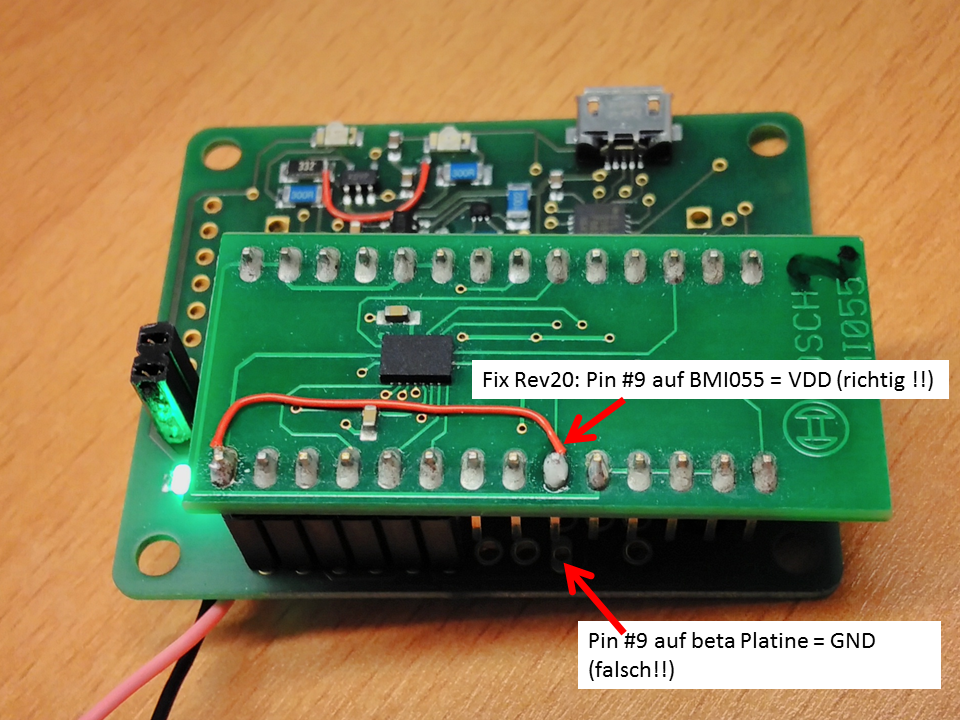
\includegraphics[width=0.835\linewidth]{images/BetaICMRev020fix}
	\caption{Übersicht mit nachträglichen Verbindungen}
	\label{fotoBeta}
\end{figure}


\clearpage
%------------------------------------------------

\subsection{Schaltplan}
Abbildung \ref{schematicBeta} zeigt den Schaltplan des Sensorboards. Zu beachten ist, dass der Sensor \emph{ICM2061 } nicht bestückt ist.\\ \textbf{$I^2C$ Betrieb}    GPIO4 = SDA und GPIO5 =SCL  
\begin{figure}[h]
	\centering
	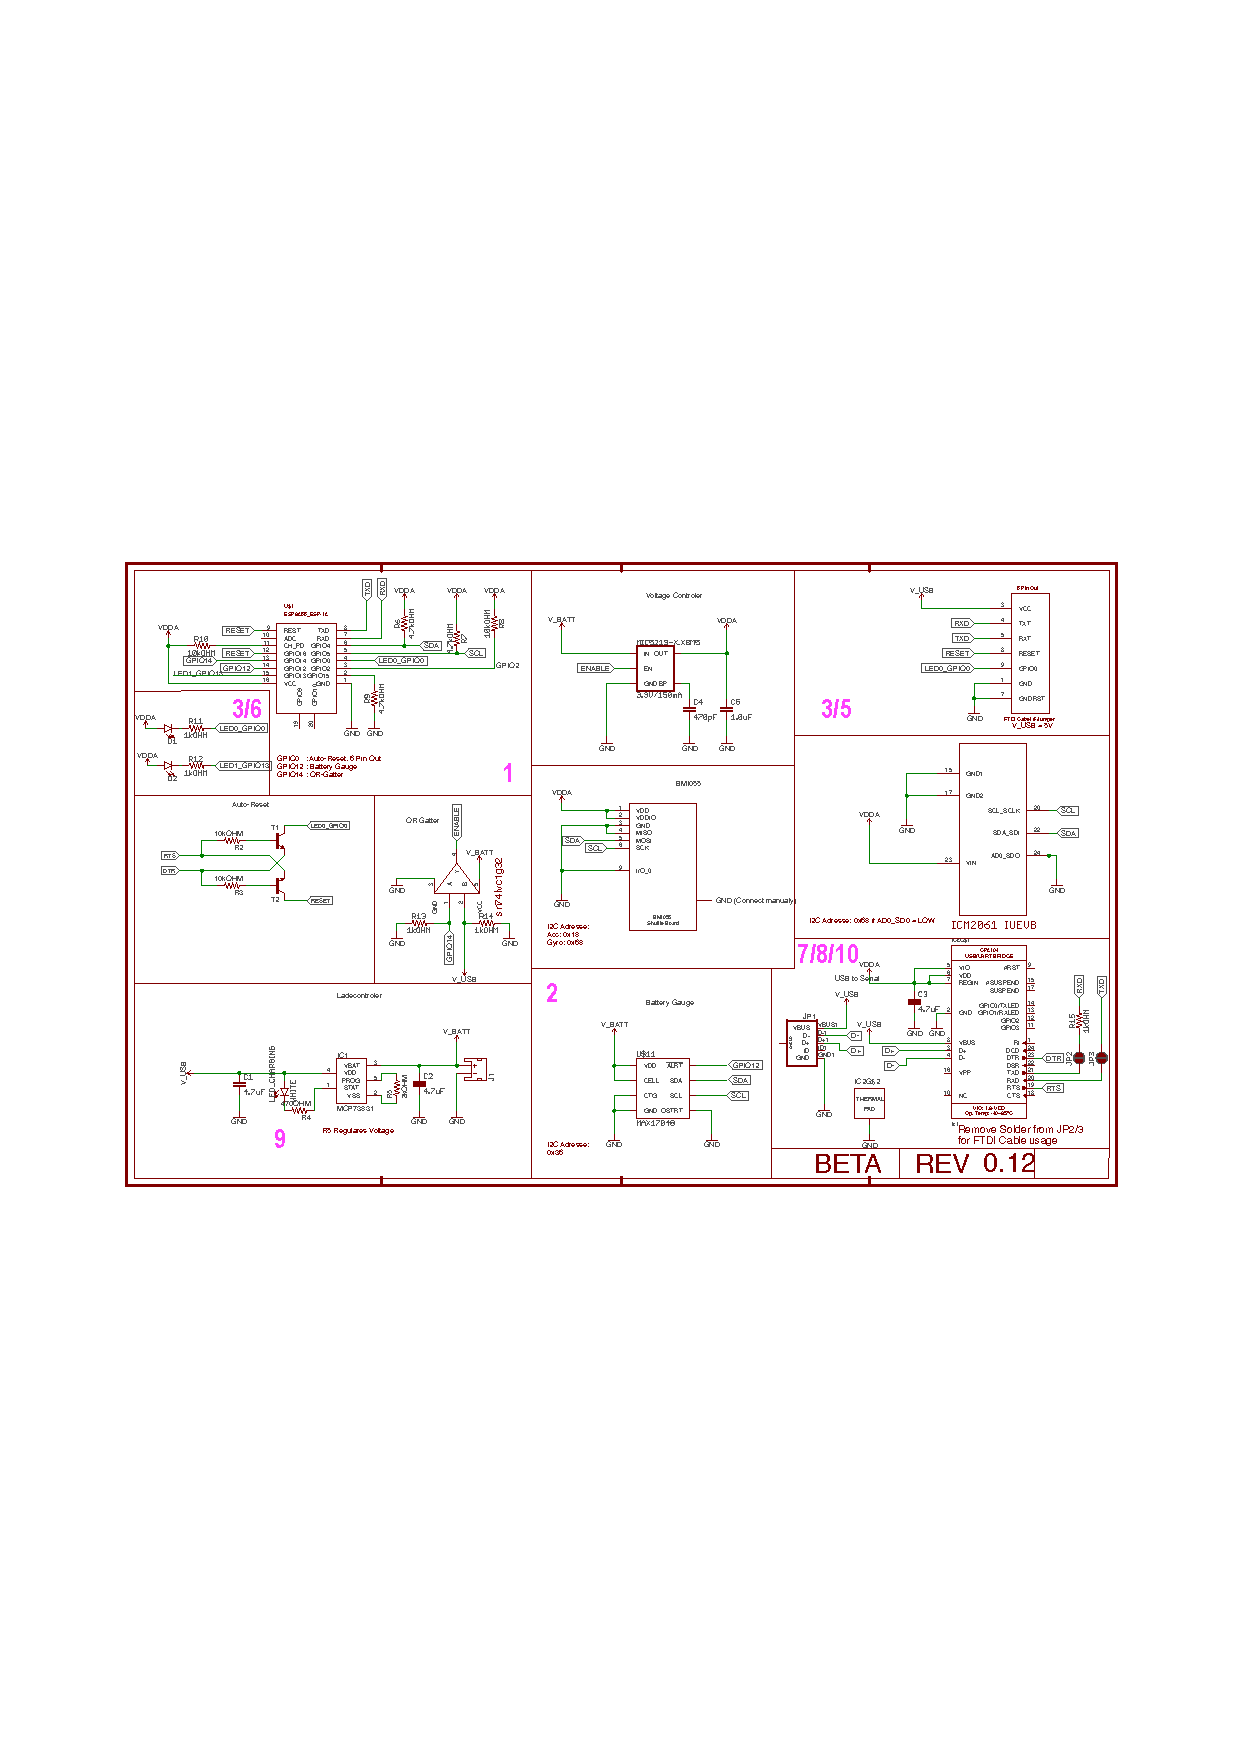
\includegraphics[width=0.935\linewidth]{images/BetaICMschRev015}
	\caption{Schaltplan des Sensorboards (ICM2061 ist nicht bestückt)}
	\label{schematicBeta}
\end{figure}

\clearpage

\subsection{Platine}
Abbildung \ref{platineBeta} zeigt die Abmessungen und den Aufbau der Platine

\begin{table}[h]
	\begin{tabular}{ll}
	
		~  & Bezeichnung\\
		\midrule
		1 & ESP-12F (\ref{ESP-12F})  \\
		2 & Fuelegauge (\ref{fuelgauge}) \\
		3 & LED D2 (\ref{LEDs})  \\
		4 & Reset (\ref{reset})  \\
		5 & FTDI Anschluss (\ref{FTDI}) \\
		6 & LED D1 (\ref{LEDs})  \\
		7 & Micro USB Anschluss  \\
		8 & CP2104 (\ref{CP2104}) \\
		9 & LED D3 (\ref{LEDs})  \\
		10 & Solderbridge (\ref{CP2104})  \\
		\bottomrule
	\end{tabular}
\end{table}

\begin{figure}[h]
	\centering
	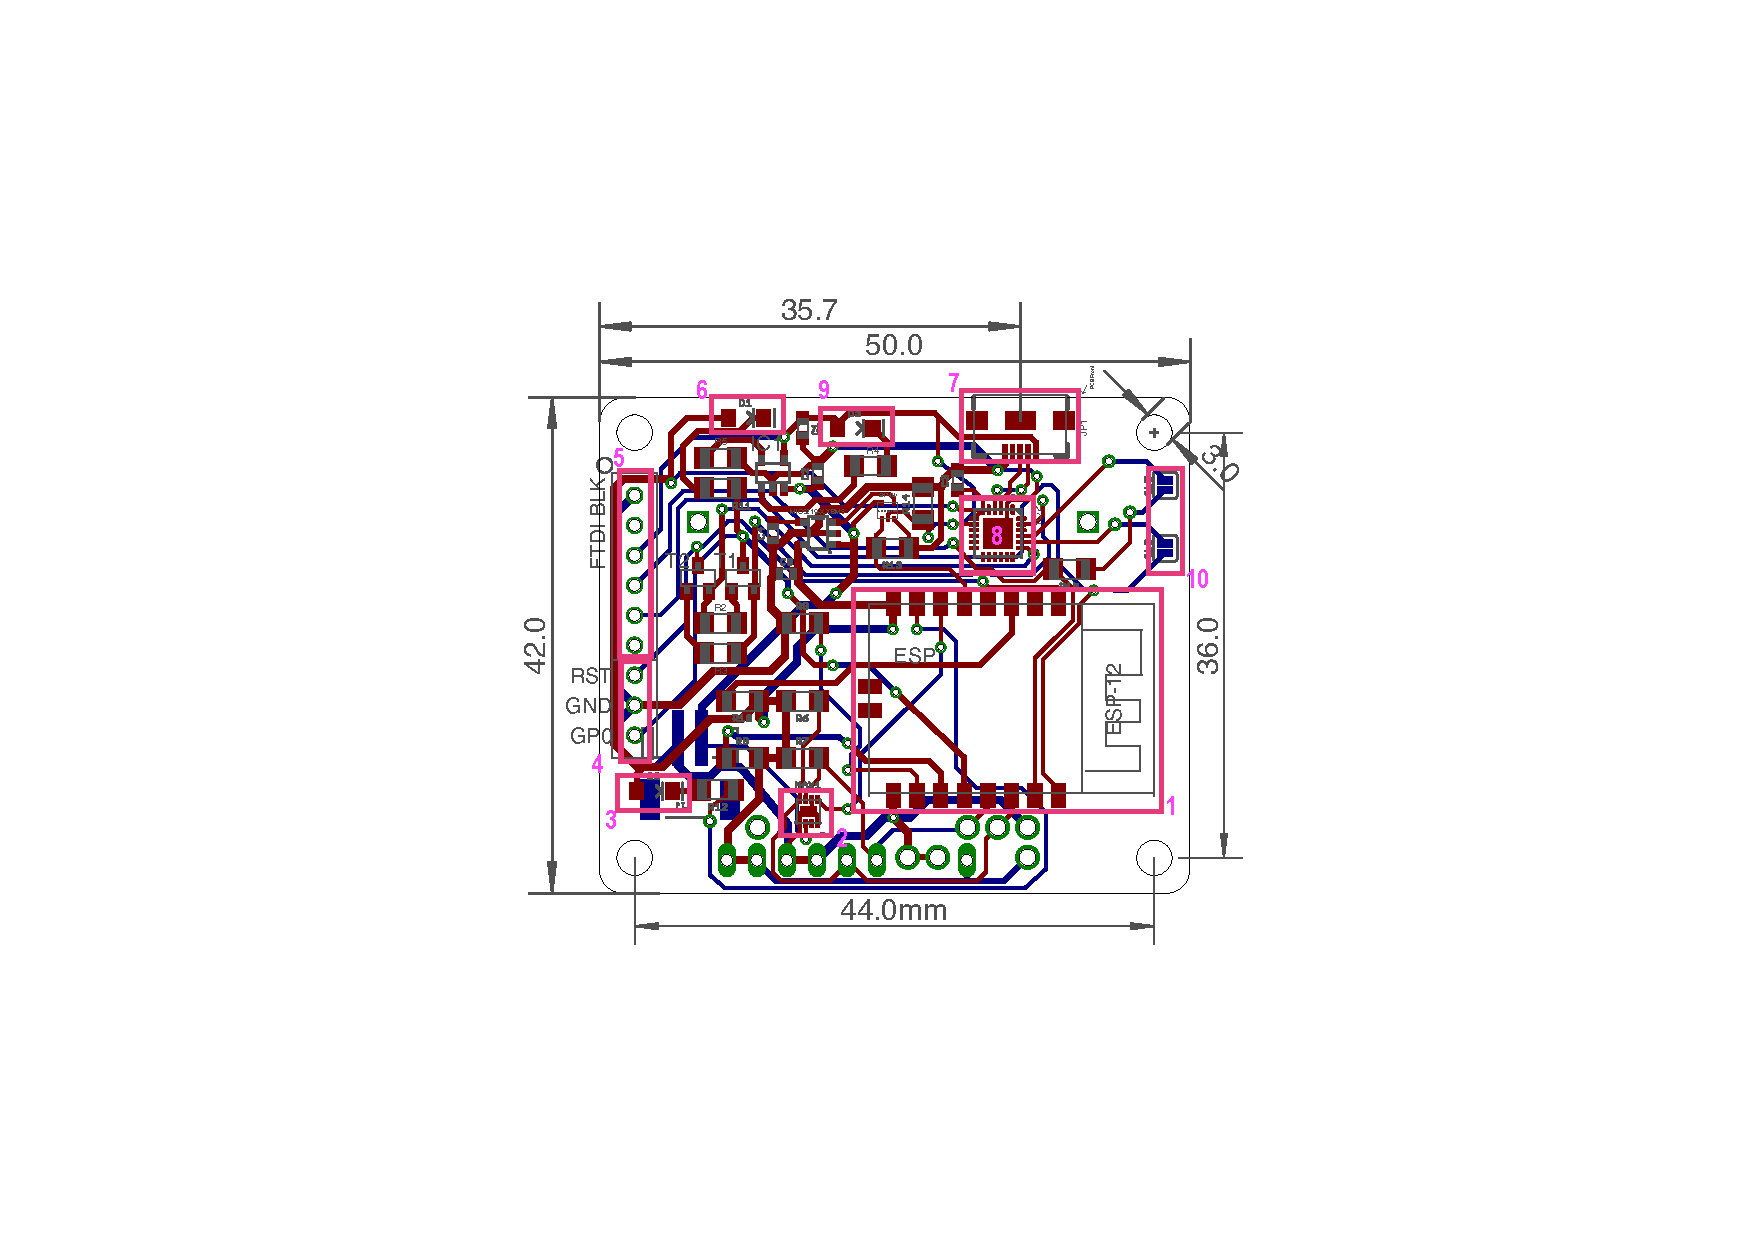
\includegraphics[width=0.735\linewidth]{images/BetaICMRev020}
	\caption{Platinen Layout ohne Sensor. \colorbox{red}{ROT}=Oben,\colorbox{blue}{Blau}=Unten, \colorbox{Green}{Grün}=Durchkontaktierung}
	\label{platineBeta}
\end{figure}



%------------------------------------------------
\clearpage

\section{Beispielanwendung} \label{Beispiele}
Im Folgenden sollen ein paar Beispiel Anwendungen gezeigt werden. Um den Code auf das Sensorboard zu \emph{Flashen} wird die Arduino IDE benötigt. Für Arduino Projekte gibt es eine große \emph{Community}, sodass die meisten Probleme durch einer kurzen Internetrecherche lösbar sind. 

\subsection{LED Test}
Der folgende Arduino Sketch testet die Funktion der LEDs.
Die Pins GPIO0 GPIO2 und GPIO13 dienen hierbei als Sink für die LED, d.h. LOW = An.\\
GPI014 muss für den Batteriebetrieb HIGH sein.
\lstinputlisting[style=Arduino]{code/Blink2LED02/Blink2LED02.ino}


\subsection{I$^2$C Scanner}

Dieser Sketch kann verwendet werden um nach über den $I^2C$-Bus angeschlossenen Sensoren zu Suchen. Im Serial Monitor der ARDUINO IDE  sollten folgende Adressen gefunden werden 0x18, 0x68 und 0x36 das sind Beschleunigungssensor \& Gyroskop (\ref{BMI055}) und Fuelgauge (\ref{fuelgauge}).


\lstinputlisting[style=Arduino]{code/i2cScanner/i2cScanner.ino}

\subsection{Übertragen des Signals via Wi-Fi}
Eine Möglichkeit die Messdaten auf einen Computer mit Matlab zu übertragen soll hier gezeigt werden.
Der Computer und der Sensor müssen imselben WiFi Netzwerk sein (z.B. WiFi-Hotspot mit Handy). Um den Sensor mit dem gewünschten Netz zu verbinden müssen im Sketch SSID und Passwort (Zeile 27-28) angepasst werden. Nach einem Reset wird über den Seriellen Monitor der Status der Verbindung angegeben. Ist der Sensor verbunden, leuchtet die grüne LED.
Das Matlab file sollte die eingehenden UDP Verbindungen Verarbeiten. 

\subsubsection{Übertragungsstruktur}
Jede Messung besteht aus 16 Byte. int32 (4 Byte) für die Zeit int16 (2  Byte) für die Beschleunigung jeder Achse und  int16 (2 Byte) für die Drehrate jeder Achse.   \\
Es werden immer 10 Messungen gemeinsam mit der Signalstärke des Wi-Fis (int32 4 Byte) und dem Ladezustand der Batterie (int8 1 Byte) übertragen, sodass das gesammte Packet $16 \cdot 10 + 5 = $ 165 Byte lang ist.\\
{\tiny 
\begin{tabular}{llllllllllllllllllllll} \toprule
	{1} & {2} & {3} & {4} & {5} & {6} & {7} & {8} & {9} & {10} & {11} & {12} & {13} & {14} & {15} & {16}& {...} &{161}& {162} & {163} & {164} & {165} \\ \midrule
	{$t_1$} & {$t_2$} & {$t_3$} & {$t_4$} & {$ax_1$} & {$ax_2$} & {$ay_1$} & {$ay_2$} & {$az_1$} & {$az_2$} &  {$ax_1$} & {$gx_2$} & {$gy_1$} & {$gy_2$} & {$gz_1$} & {$gz_2$}& {...} & {$wifi_1$} & {$wifi_2$} & {$wifi_3$} & {$wifi_4$} & {bat}\\  \bottomrule
\end{tabular}}
 {\normalsize }\\
 
 Die Werte werden im Matlab Skript  (Zeile 40-50) zusammengesetzt.
\subsubsection{Matlab Code}

\definecolor{gray}{rgb}{0.95,0.95,0.95}
\definecolor{mgreen}{rgb}{0.1,0.5,0.1}  %Matlab-Grün
\lstset{
	breaklines=true,
	inputencoding="latin1",
	backgroundcolor=\color{gray},
	basicstyle=\scriptsize\ttfamily,
	commentstyle=\color{mgreen}\ttfamily,
	emph={square}, 
	emphstyle=\color{blue}\texttt,
	emph={[2]root,base},
	emphstyle={[2]\color{yac}\texttt},
	showstringspaces=false,
	flexiblecolumns=false,
	tabsize=4,
	numbers=left,
	numberstyle=\tiny,
	numberblanklines=false,
	stepnumber=1,
	numbersep=10pt,
	xleftmargin=15pt
}
\lstinputlisting[language=matlab]{code/betareadout/betareadout.m}

\subsubsection{ Arduino Sketch}
Dieser Sketch 
\lstinputlisting[style=Arduino]{code/test_BETA/test_BETA.ino}



\section{Komponenten}

\subsection{ESP-12F}
\label{ESP-12F}
Das ESP8266 Modul ist ein Ultra-low-Power-32-Bit-Mikrocontroller.  Integriertes WLAN ermöglicht die Kommunikation nach Außen.  
Die Programmierung kann z.B. über die ARDUINO-IDE vorgenommen werden. Die Sensoren (IMU, Batteriestand) sind über einen $I^2C$-Bus angeschlossen.
\begin{description}
	\item[WiFi Protocles] 802.11 b/g/n
	\item[Frequency Range ] 2.4GHz-2.5GHz (2400M-2483.5M)
	\item[Security] WPA/WPA2  WEP/TKIP/AES
	\item[Stromverbrauch] 80 mA
	\item[Network Protocols] IPv4, TCP/UDP/HTTP/FTP
\end{description}
\subsection{BMI055}
\label{BMI055}
Der BOSCH BMI055 ist eine Inertiale Messeinheit (IMU) und somit  eine räumliche Kombination von Beschleunigungssensoren  und Drehratensensoren. Die Messungen erfolgen in x-, y- und z- Richtung und realisieren so  6 Freiheitsgrade (6DoF). 

\paragraph{Accelerometer}
\begin{description}
	\item[I2C Adresse] 0x18
	\item[Auflösung] 12bit
	\item[Messbereich ] Programmierbar:  ±2g/±4g/±8g/±16g
	\item[Stromverbrauch] 130 $\mu$A
\end{description}
\paragraph{Gyroskop}
\begin{description}
\item[I2C Adresse] 0x68
\item[Auflösung] 16bit
\item[Messbereich ] Programmierbar:  ±125°/s to ±2000°/s
\item[Stromverbrauch] 5mA 
\end{description}
\subsection{Fuelgauge}
\label{fuelgauge}
Der Batteriestandsanzeiger MAX17048 bietet die Möglichkeit den Ladestand eines LiPo-Akkus (1 Zelle, 3.7V) in Prozent abzufragen.  Interne wird die Spannung in eine einem Model in Prozent umgerechnet, dabei werden spezifische Effekte der Batterie, wie Temperatur und Spannungskurve berücksichtigt.
\begin{description}
		\item[I2C Adresse] 0x36
	\item[Precision]  ±7.5mV
	\item[Stromverbrauch] <23$\mu$A
\end{description}

\subsection{LEDs}
\label{LEDs}
Das Board verfügt über 3 LEDs von denen 2 über die GPIOs des ESP8266 Moduls frei programmierbar sind. Eine LED ist als Ladeindikator vorgesehen.

\begin{table}[h]
	\caption{LEDs}
	\centering
	\begin{tabular}{llr}
		Name & Anschluss & Farbe \\
		\midrule
		D1 & GPIO0 & ??? \\
		D2 & GPIO13 & ??? \\
		D3 & Ladestand & ??? \\
		\bottomrule
	\end{tabular}
\end{table}

LED D1 blinkt wenn Kommunikation über die UART Schnittstelle stattfindet.

\subsection{CP2104 }
\label{CP2104}
CP2104 Chip als USB/UART Bridge für die Programmierung. Treiber sind für alle gängigen Betriebssystem vorhanden. RXD und TXD können ggf. manuell getrennt werden (Siehe \emph{Solderbridge} Abb. \ref{platineBeta}).

\subsection{FTDI Anschluss }
\label{FTDI}
Anschluss für 5 Volt FTDI Kabel (GND, CTS, VCC, TXD, RXD, RTS). Kann auch zum laden des Akkus verwendet werden.

\subsection{Reset}
\label{reset}
\blindtext

\section{Anhang}
\subsection{Bibliotheken}
\subsubsection{BMI055}
\lstinputlisting[style=arduino]{code/test_BETA/BMI055.cpp}
\subsubsection{BMI055.h}
\lstinputlisting[style=arduino]{code/test_BETA/BMI055.h}


\subsubsection{I2Cdev}
https://github.com/jrowberg/i2cdevlib/blob/master/Arduino/I2Cdev/I2Cdev.h
\subsubsection{MAX17048}
https://github.com/libpropeller/libpropeller/blob/master/libpropeller/max17048/max17048.h
%----------------------------------------------------------------------------------------
%	BIBLIOGRAPHY
%----------------------------------------------------------------------------------------
\printbibliography[title={Datenblätter}] % Print the bibliography, section title in curly brackets

%----------------------------------------------------------------------------------------

\end{document}
